%\documentclass[PhD,two side]{srmuthesis}
%\documentclass[MS]{srmuthesis}
%\documentclass[MTech]{srmuthesis}
\documentclass[BTech]{srmuthesis}
\usepackage[dvipsnames]{xcolor}
\usepackage{times}
\usepackage{t1enc}
\usepackage{tikz}
\usepackage{subfigure}
\usepackage{pgfplots}
\usepackage{setspace} 
\usepackage{geometry}
\usepackage{graphicx}
\usepackage{epstopdf}
\usepackage{lscape}
\usepackage{fancyhdr}
\usepackage{natbib}
\usepackage{hyperref} % hyperlinks for references.
\usepackage{amsmath} % easier math formulae, align, subequations \ldots
\usepackage{amssymb}
\usepackage{wasysym}
\usepackage{titlesec}
\usepackage{textcomp}
\usepackage{pifont}
\usepackage{appendix} 
\usepackage{listings}
\usepackage{graphicx}
\usepackage{indentfirst}
\usepackage[section]{placeins}
\usetikzlibrary{decorations.pathmorphing}
\usetikzlibrary{shapes,arrows,shadows,patterns}
\usepackage[printonlyused]{acronym}
\usepackage{array}
\newcolumntype{L}{>{\centering\arraybackslash}m{4cm}}
\graphicspath{ {content/} }
\usepackage{color}
\definecolor{lightgray}{rgb}{.9,.9,.9}
\definecolor{darkgray}{rgb}{.4,.4,.4}
\definecolor{purple}{rgb}{0.65, 0.12, 0.82}


\lstdefinelanguage{JavaScript}{
	keywords={typeof, new, true, false, catch, function, return, null, catch, switch, var, if, in, while, do, else, case, break},
	keywordstyle=\color{black}\bfseries,
	ndkeywords={class, export, boolean, throw, implements, import, this},
	ndkeywordstyle=\color{darkgray}\bfseries,
	identifierstyle=\color{black},
	sensitive=false,
	comment=[l]{//},
	morecomment=[s]{/*}{*/},
	morestring=[b]',
	morestring=[b]"
}

\lstset{
	language=JavaScript,
	extendedchars=true,
	basicstyle=\footnotesize\rmfamily,
	showstringspaces=false,
	showspaces=false,
	tabsize=2,
	breaklines=true,
	showtabs=false,
	captionpos=b
}





%\usepackage{nomencl}
%\newcommand{\bigsize}{\fontsize{16pt}{20pt}\selectfont}
%\renewcommand\nomname{\centerline {NOTATION}}
%\makenomenclature
\setcounter{MaxMatrixCols}{20}
\begin{document}
%%%%%%%%%%%%%%%%%%%%%%%%%%%%%%%%%%%%%%%%%%%%%%%%%%%%%%%%%%%%%%%%%%%%%%
% Title page

\title{ARtichect: AR based Construction Simulator} % Enter The Project Title

\firstauthor{Vijay Krishna V}% Enter The Student name
\firstauthorregno{[Reg No: RA1511003020329]}
\secondauthor{Sai Kiran Reddy L}% Enter The Student name
\secondauthorregno{[Reg No: RA1511003020359]}
\thirdauthor{Krishna Reddy M} % If there is no third author, leave the space blank like \thirdauthor{}
\thirdauthorregno{[Reg No: RA1511003020332]}
\fourthauthor{Satish Kumar L}
\fourthauthorregno{[Reg No: RA1511003020384]}
\guide{ Mrs Elakya R } % Enter your guide's name
\designation{ Asst. Professor } % Enter your guide's designation
\guidedepartment{Computer Science \& Engineering} % Enter the department name of your Guide 
\hod{Dr. JAGADEESAN,M.Tech.,Ph.D} % Enter HOD's name
\department{Computer Science \& Engineering} % Enter your department name
\date{MAY 2018} % Enter month and year of submission
%\nocite{*}

\maketitle
%%%%%%%%%%%%%%%%%%%%%%%%%%%%%%%%%%%%%%%%%%%%%%%%%%%%%%%%%%%%%%%%%%%%%%
%\vspace*{3in}
%\begin{center}
%{\Huge Dedicated to my Parents}
%\end{center}
%%%%%%%%%%%%%%%%%%%%%%%%%%%%%%%%%%%%%%%%%%%%%%%%%%%%%%%%%%%%%%%%%%%%%%
% Certificate
\certificate

%\vspace*{0.5in}



%%%%%%%%%%%%%%%%%%%%%%%%%%%%%%%%%%%%%%%%%%%%%%%%%%%%%%%%%%%%%%%%%%%%%%
% Abstract


\abstract
\begin{doublespacing}
\large\noindent 
Augmented reality (AR) is a technology that combines the physical and digital worlds together. AR provides a rich and immersive experience as the real-world surroundings of the user becomes interactive and digitally manipulatable. In this paper, a user-friendly, portable and platform independent AR system   is proposed that allows users to manipulate/construct 3D virtual buildings on a real tabletop using Web-AR so that it is accessible to everyone anywhere. Since it is virtual, they are also free to interact with the model in real time by adding or deleting parts to the building or scaling portions of it to examine in greater detail. Simulated tests like structural integrity, Air Flow and Lighting can be performed on this virtual model.This project aims to make 3D modelling of a building easier by providing a natural and more intuitive interaction. It makes use of the inbuilt camera to map the digital objects into the real world with the help of markers and JavaScript libraries/frameworks like Three.js, AR.js and A-Frame.js. AR places digital objects and useful information into the real world, which has the potential to make our phones more intuitive and helpful\\
\end{doublespacing}

% Table of contents etc.

\begin{singlespace}
\tableofcontents

\listoftables
\addcontentsline{toc}{chapter}{LIST OF TABLES}
\listoffigures
\addcontentsline{toc}{chapter}{LIST OF FIGURES}
\end{singlespace}


%%%%%%%%%%%%%%%%%%%%%%%%%%%%%%%%%%%%%%%%%%%%%%%%%%%%%%%%%%%%%%%%%%%%%%

\abbreviations
%\begin{acronym}[longest acronym must be entered here]
\begin{acronym}[OKID/ERA]

%\acro{acronym}{in detail}
\acro{API}{Application program interface}
\acro{AR}{Augmented Reality}
\acro{REST} Representational Stateless Transfer
\acro{JSON}{Java Script Object Notation}
\acro{JS}{Java Script}
\acro{SQL}{Standardized Query Language}

\end{acronym}
% Use the syntax \ac{acronym} whereever you use this acronym.
% Abbreviations


\pagebreak

% The main text will follow from this point so set the page numbering
% to arabic from here on.
\pagenumbering{arabic}


%%%%%%%%%%%%%%%%%%%%%%%%%%%%%%%%%%%%%%%%%%%%%%%%%%
% Introduction.

%Enter your chapter number here
\chapter{Introduction}
\section{Overview}
Augmented reality (\ac{AR}) is a growing phenomenon, it  is used to enhance the natural environments or situations and offer perceptually enriched experiences. With the help of advanced AR technologies the information about the surrounding real world of the user becomes interactive and digitally manipulable.

The primary value of augmented reality is that it brings components of the digital world into a person's perception of the real world, and does so not as a simple display of data, but through the integration of immersive sensations that are perceived as natural parts of an environment.

Augmented reality is incredibly useful for solving everyday problems. Put furniture into your space to see how it looks and fits in your home. Or navigate complicated spaces without ever looking at a map. Now, you can do things you couldn't imagine before using augmented reality, and discover new ways of doing the things you need to get done today. 

With augmented reality, the entire world around you is in play. Bring virtual monsters to life in your neighborhood park or on your kitchen counter. Or put on a mask to instantly join a costume party with friends halfway across the globe. By interacting with virtual objects as if they're in your surroundings, you can immerse yourself in entertainment like you never imagined.

Firsthand experience is one of the most powerful ways to learn. And with augmented reality, you can experience just about anything you can imagine. Break down the complicated mechanics of a car engine before touching a wrench. Or analyse the most minute bones of the human body without making a single incision. The possibilities for learning are virtually limitless.

Applications of augmented reality can be as simple as a text-notification or as complicated as an instruction on how to perform a life-threatening surgical procedure. They can highlight certain features, enhance understandings, and provide accessible and timely data. Cell phones apps and business applications by companies using augmented reality are a few of the many applications driving augmented reality application development. The key point is that the information provided is highly topical and relevant to what you want you are doing.

\section{Problem Statement}
Augmented reality and virtual reality are redefining the way in which we communicate, shop, and interact with each other. While this technology may not be new, it has improved a thousand times over the last few decades, and continues to excite users with the new ways in which the lines are blurred between computer generated technology and real-life. Although AR has many advantages some of the main drawbacks that are yet to be addressed are:
\begin{itemize}
\item \textbf{Invades Privacy -} Just like other modern technologies on the market, AR \& VR can be prone to data hacks as well - and that's a scary thing, considering how much data is connected to virtual environments. Many people also fear the way in which personal data might be used by authorities in order to track or control individuals.
\item \textbf{Hampers Interaction With Real-World -}
If one can see and experience the world from your living room, would you ever really need to leave the house? AR and VR may provide new ways for people to communicate, but they could also possibly take away an important aspect of our social life that involves around human interaction.

\item \textbf{A Good Use Case -} The biggest unsolved problem today in the AR space is that it is still lacking an everyday killer application.

\item \textbf{Poor Experience -} in action, it always seems lackluster. Whether it's poor resolution, inaccurate computer vision, or uncomfortable human/computer interactions, the actual experience never lives up to what it's supposed to be.

\item \textbf{Exposure to AR -} Consumers aren't exposed to AR regularly and don't see its wide-reaching applications in their daily lives.

\end{itemize}
These drawbacks will be addressed by the project, We've developed
it using Web Technologies so that it can run on any device
that has a web browser and is not limited by OS or Hardware.
Since it is a web application no installation is required and
can be accessed anywhere. The project will be implemented to address all the drawbacks of the existing system and improvise the effectiveness of the system.
\section{Objective}
This project is related to the upcoming or rather latest technology called Augmented Reality. Augmented reality is a powerful way to bring the physical and digital worlds together. AR places digital objects and useful information into the real world around us, which creates a huge opportunity to make our phones more intuitive, more helpful and a whole lot more fun.

This project proposes an idea to visualize the effect of natural calamities on structures and offers an in-depth analysis of the structural weak points of a design. With AR, Instead of displaying the blueprints of architectural design on a 2-D board or on auto-cad we can visualize the 3-D models in a real-time environment where it can be interacted by the user. Currently, AR applications focus mainly on the construction and alignment of objects in the real-world environment, This proposal takes that concept one step further by performing realistic simulations of the natural calamities such as floods,  drought, wind, lighting and effect of rain on the structural and materialistic properties of the simulated designs by using a particle-based physics engine. 

At present, the effect of natural calamities might sometimes turn out to be incalculable when estimating the human and structural loss. The damage can be partially prevented by designing a near to perfect structure that is able to withstand the calamities in a realistic physics simulation. Thus simulations not only help in estimating the damage but can also help us to prevent the disasters to an extent. In this proposal, the simulation of natural phenomenon such as Hurricanes, Earthquakes and Lightning on the materialistic and structural properties of the design can help in detecting the flaws in a design.

The alignment and design of AR-based models according to real-time scenarios requires precision and correctness. The tools used in designing such effective structural designs and simulations are three.js, AR.js, A-Frame, Tracking.js (\ac{JS} libraries). The various user interactive formats proposed in the design are Gesture Recognition, Marker Tracking, 3D Object Interaction, 3D Scene Rendering.
ARCore will be used to integrate this into an Android application. This will be done after the completion of the web application. This will be a basis to other major Applications that will actually help people. And hence this project will be a learning platform to launch into other more useful projects!
\section{Organization of the report}
There are five chapters in the report of the project ARtifact - Augmented Reality On The Web. The domain of the project is Augmented Reality. The report gives a comprehensible overview of the design and implementation details of the project, it helps understand the various technologies used in the project and the effective implementation of these technologies.
 
\subsection*{Chapter 1}
This chapter gives the basic introduction of the project, it gives the basic overview of the entire project and gives the details about the problem statement and the main objective of the project.

\subsection*{Chapter 2}
This chapter includes the literature survey which is a survey done on various base papers, it mainly gives the problems and conclusions for the domain of the project. The chapter also gives the description about  all the features of the existing system and its drawbacks and the proposed system and its advantages.

\subsection*{Chapter 3}
This chapter gives the requirements of the project in detail. It includes the basic purpose of the project, its scope, user requirements of the project. Software and Hardware specifications required by the project are given in detail in this chapter.

\subsection*{Chapter 4}
This chapter the complete information about the system design and the various modules present in the project. The chapter gives the system architecture and its description , it gives the detailed description about the data flow diagram. The module implementation is given in detail with the screen shots from the projects and the diagrams required. Data flow diagram and the process description for each module is separately given for better understanding.

\subsection*{Chapter 5}
This chapter deals with entire implementation of the system. The information about the platform of the project is given, the sample coding and the screen shots of the working model with proper description is given this chapter. The project will be done and the summary will be given.
\subsection*{Chapter 6}
The system implementation of the project will be given in this chapter. The project also gives an insight
about the implementation details,technologies used.
\subsection*{Chapter 7}
The conclusion of the project will be given in this chapter.The project also gives an insight about the future work which can be implemented through the project.

\chapter{Literature Survey}
\section{Introduction}
In this section we're going to talk about the various papers we have looked at which are related to our project.
\section{Existing System}
%TODO Autocite References Using BibLaTex

\paragraph{Virtual object manipulation on a table-top AR environment} by (\cite{tabletop})
The AR interface helps in manipulating 3-D virtual objects
over a table top. Several architects can sit around a table to
design a plan for the building that is about to be constructed.
Here through HMD displays they can see their plans in 3-D
projections. The 3-D models are mapped to the real environ-
ment. This helps in face to face collaboration where they can
design virtual scenes and experience them immersively. It also
helps to overcome real life obstacles at the time of creation
and planning.It also addresses the problems of virtual object interaction and user tracking in a table-top AR interface such as Accuracy, Robustness and an intuitive interface.

\paragraph{Introduction of Physics Simulation in AR} by (\cite{introphysics})
The augmented reality is an environment where it has both
virtual and real objects simultaneously. So it is necessary to
describe the object with accurate properties. The motion of
virtual objects in virtual reality may be less attractive and is
hard for AR objects to be perceived as real. This gap can be
reduced by using different physics engines. This helps in visualizing
real-world scenarios where these engines can be used
to detect daily routines for rigid bodies, particles, dynamics,
collision detection, havoc engine for havoc detections

\paragraph{3D interaction techniques using gestures recognition in virtual environment} by (\cite{gestureinteraction})
Nowadays with the use of smart phones touch screens have
become popular but they have limited functionality. Use of the
hand gestures is an interesting way to interaction with the AR
environment as the experience is more natural and intuitive.
Here the AR environment can be manipulated by hand gesture
recognition techniques\cite{gestureinteraction}. cyberglove is a tool that can be
used to record and obtain information on hand motions.
GRT(gesture recognition toolkit) also helps in receiving these
hand motion data from the given input signals. The interaction
techniques are mostly by gestures like direction, placement etc.

\paragraph{AR for construction site monitoring and documentation} by (\cite{sitemonitoring})
The growth in the use of AR has eased the study and development in various fields. The demands for documentation of work progress and its physical visualization has been increased. Using 3-D reconstruction and aerial monitoring the physical environment has been captured and the progress of the work can be seen where the physical data is projected into the system or the devices with clients for on-site visualization using AR. Augmented reality ( is an interface that overlays digital information onto the user's view, spatially aligned to the current physical environment. The user's view is often a camera image of their physical surroundings. The video image is augmented with digital information and rendered on the display device. Such an overlay allows for the presentation of information that is relevant to a specific task right on site and aligned to the objects of interest.

\paragraph{The research and application of AR technology} by (\cite{researchar})
AR utilizes virtual information generated by the computer
to mix with the real environment users observe. The real
environment and virtual reality timely add to the same scene
or space co-exist, expanding and augmenting the perception of
users with the world around. AR provides the information that
is different from the information human can sense in general
condition, which can help in many real world scenarios.
Through the related research and analysis, three dimensional
tracking registration, real-time human-computer
interaction and virtual reality fusion are the key techniques to
affect the performance of AR system. With the continuous
development of virtual reality technology, especially from
the laboratory stage to the practical application, its impact is
increasingly significant.


\paragraph{Augmented Reality for Board Games} Talks about turning a standard real game board pawns into an AR game. Using the objects as a tangible interface, and augment them with visual effects. The game logic can be performed automatically by the computer. This results in a better immersion compared to the original board game alone and provides a different experience than a video game.

One trend we are seeing more and more of is the use of interactive video content - 360 videos, Augmented and Virtual Reality - the next progressive step from video providing an interactive customer experience. Now with Apple creating animojis, it seems like the first step (on a small scale) to animating yourself and sharing content in this interactive and creative way. Each of the mentioned papers provides an incremental upgrade in the field of AR technology and brings new ways of user interaction that is immersive and natural.

\section{Issues in Existing System}
AR faces a tough road. Nothing will happen overnight and there's still a chance AR fails, but when you break it down into individual threats, you can see that most are capable of being overcome. The technology is still in its early stages and brands are still feeling their way around it. That  being said, many of the most innovative and forward-thinking brands have begun to integrate AR into their campaigns

\subsubsection{Poor Experience} The concept of AR is cool and useful, in action, it always seems lackluster. Whether it's poor resolution, inaccurate computer vision, or uncomfortable human/computer interactions, the actual experience never lives up to what it's supposed to be.

At the moment, the resolution is too low on top of the fact that it's not fully immersive and it makes people nauseous. Similar issues are abundant in development edition AR headsets. Although it is understood that this is still early days, the experience seems so far away that maybe what we dream of is still a technological wave away.


\subsubsection{Lack of consumer exposure}
One of the most difficult challenges about AR is educating the broader market.  Consumers aren't exposed to AR regularly and don't see its wide-reaching applications in their daily lives. However, there are plenty of AR experiences available today that just lack exposure in the consumer market.  

At present Augmented Reality is still being used primarily for entertainment and advertising, as this changes and it expands into education, medicine, maintenance, and other fields that are always looking for more effective methods or solutions it's likely that AR will become a regular option in our lives.

Also, it is important to build a strong pipeline of rising talent in the AR/VR community to continue to innovate and develop this technology. It is critical that students have exposure to this technology in the classroom. It is easy to be intimidated by emerging tech, but with early exposure, AR/VR can become more accessible.  
\subsubsection{The risk of physical safety}
The primary social challenge is that a regular mobile phone is currently a serious distraction for motorists during driving, accounting for numerous road accidents each year. And AR applications that provide drivers with directions have both clear benefits and drawbacks as well. When dealing with a mixed reality, accidents are bound to happen.

Displaying the relevant traffic-monitoring cam feeds and all sorts of additional information, the AR app requires drivers to pay attention to their mobile devices instead of the road ahead. Considering the effect mobile phone usage has on driving, it is not hard to imagine a driver becoming overwhelmed with information in this instance. This is how AR can easily distract you from reality.
\subsubsection{Expensive Hardware}
Today, no AR headsets are available for consumers. Microsoft HoloLens and Meta 2 have released developer versions, but they have not yet announced when we can expect their devices to ship to consumers. Even more, HoloLens and Meta still boast hefty price tags at \$3,000 and \$949, respectively.

As we wait for smart headsets to hit the consumer market, AR must be experienced through our mobile devices. To make a long story short, dedicated augmented reality devices are not consumer-ready yet. Alongside that, there is still the issue of device interoperability and authoring limitations based on specific platforms. We've been waiting for smart augmented reality headsets to hit the consumer market for quite some time now, but they are still a few years away. This means our mobile devices remain the only viable tools able to stimulate AR adoption.Yet, most of current mobile devices are not well-suited for this purpose. The issue with most of our smartphones/tabs/whatever is that they are not featured with technologies like room mapping or depth sensing.

\section{Summary of Literature Survey}
Currently, Augmented Reality remains widely unknown to the general public and in order to change this, an AR app development company has to create a rich variety of user experiences that are functional, reasonable, and have an easy learning curve.
\subsection{Proposed system}
Augmented reality is a powerful way to bring the physical and digital worlds together. AR places digital objects and useful information into the real world around us, which creates a huge opportunity to make our phones more intuitive, more helpful and a whole lot more fun.
\subsubsection{ARchitect - AR based Construction Simulation}
This project proposes an idea to visualize the effect of natural calamities on structures and offers an in-depth analysis of the structural weak points of a design. With AR, Instead of displaying the blueprints of architectural design on a 2-D board or on auto-cad we can visualize the 3-D models in a real-time environment where it can be interacted by the user. Currently, AR applications focus mainly on the construction and alignment of objects in the real-world environment, This proposal takes that concept one step further by performing realistic simulations of the natural calamities such as floods,  drought, wind, lighting and effect of rain on the structural and materialistic properties of the simulated designs by using a particle-based physics engine. 

At present, the effect of natural calamities might sometimes turn out to be incalculable when estimating the human and structural loss. The damage can be partially prevented by designing a near to perfect structure that is able to withstand the calamities in a realistic physics simulation. Thus simulations not only help in estimating the damage but can also help us to prevent the disasters to an extent. In this proposal, the simulation of natural phenomenon such as Hurricanes, Earthquakes and Lightning on the materialistic and structural properties of the design can help in detecting the flaws in a design.

\chapter{Specifications}
\section{Introduction}
In this chapter, the specifications of this project are going to be discussed in detail. Topics like purpose, project scope and much more is also included.
\subsection{Purpose}
In the present day scenario, There is an increase in the use of AR technology in both commercial and industrial applications, many companies are adopting the new vision towards designing of their products using AR and VR which not only reduces the designing cost but also helps in the testing of many real-time scenarios and provides a natural interaction that is easy to use.

Ford is using the AR technology in visualizing the structural design of the new cars and is also using the simulated effects of wind and snow on 
the engine performance, Space travel revolutionizing company Space-x simulates the effect of gravity and rockets orbit placement using AR, 
The Boeing is using AR to design the new Air Force One in which it simulates the effects of engine propulsion , and also for the core structure designing which is a heavy in-built metal body to withstand any missile attacks on the plane. Thus simulation plays a major role in designing a product where the imperfections can be detected and rectified in the early stages of development and help the company to create a final product that is robust and reliable.

This paper proposes an idea to visualize the effect of natural calamities on structures and offers an in-depth analysis of the structural weak points of a design. With AR, Instead of displaying the blueprints of architectural design on a 2-D board or on auto-cad we can visualize the 3-D models in a real-time environment where it can be interacted by the user. Currently, AR applications focus mainly on the construction and alignment of objects in the real-world environment, This proposal takes that concept one step further by performing realistic simulations of the natural calamities such as floods,  drought, wind, lighting and effect of rain on the structural and materialistic properties of the simulated designs by using a particle-based physics engine. 

At present, the effect of natural calamities might sometimes turn out to be incalculable when estimating the human and structural loss. The damage can be partially prevented by designing a near to perfect structure that is able to withstand the calamities in a realistic physics simulation. Thus simulations not only help in estimating the damage but can also help us to prevent the disasters to an extent. In this proposal, the simulation of natural phenomenon such as Hurricanes, Earthquakes and Lightning on the materialistic and structural properties of the design can help in detecting the flaws in a design.

\subsection{Project Scope}
At present, the effect of natural calamities might sometimes turn out to be incalculable when estimating the human and structural loss. The damage can be partially prevented by designing a near to perfect structure that is able to withstand the calamities in a realistic physics simulation. Thus simulations not only help in estimating the damage but can also help us to prevent the disasters to an extent. In this proposal, the simulation of natural phenomenon such as Hurricanes, Earthquakes and Lightning on the materialistic and structural properties of the design can help in detecting the flaws in a design.
\section{Overall Description}
In overall description we're going to discuss about how the project is implemented. Description of what was done, the features, the user characteristics, operating environment, implementation constraints and much more.
\subsection{Product Features}
The various feature in our web application will include the following:
\begin{itemize}
% TODO add some features %
\item\textbf{Immediacy:} Mobile Websites Are Instantly Available 
A mobile website is instantly accessible to users via a browser across a range of devices (iPhone, Android, BlackBerry, etc).  Apps on the other hand require the user to first download and install the app from an app marketplace before the content or application can be viewed - a significant barrier between initial engagement and action/conversion. 
\item\textbf{Compatibility:} Mobile Websites are Compatible Across Devices
A single mobile website can reach users across many different types of mobile devices, whereas native apps require a separate version to be developed for each type of device. Furthermore, mobile website URLs are easily integrated within other mobile technologies such as SMS, QR Codes and near field communication (NFC).
\item\textbf{Upgradability:}  Mobile Websites Can Be Updated Instantly
A mobile website is much more dynamic than an app in terms of pure flexibility to update content. If you want to change the design or content of a mobile website you simply publish the edit once and the changes are immediately visible; updating an app on the other hand requires the updates to be pushed to users, which then must be downloaded in order to update the app on each type of device. 
\item\textbf{Findability:} Mobile Websites Can be Found Easily
Mobile websites are much easier for users to find because their pages can be displayed in search results and listed in industry-specific directories, making it easy for qualified visitors to find you. Most importantly, visitors to your regular website can be automatically sent to your mobile site when they are on a handheld (using device-detection).  In contrast, the visibility of apps are largely restricted to manufacturer app stores.
\item\textbf{Reach:} Mobile Websites Have Broader Reach
Because a mobile website is accessible across platforms and can be easily shared among users, as well as search engines, it has far greater reach capability than a native app. 
\end{itemize}
\subsection{User classes and characteristics}
The various user classes and their characteristics are given below:

\subsubsection{Login}
The login class takes the login information from the user and authenticates it. If the information matches with that of the database..                          
\subsubsection{Menu}
The menu is where the user can select what functionality he/she wants to use. The various menu items include:
\begin{itemize}
\item Object placement tool
\item Physics Simualation parameters
\item Perform Tests
\item Structural Analysis
\end{itemize}

\subsubsection{Object placement tool}
This is where the user can place a virtual object in the scene to construct a building or structure.
\subsubsection{Physics Simualation parameters}
Control the intensity of physics engine and simulation.  
\subsubsection{Perform Tests}
perform various tests on the building to get a better idea of its structural integrity
\subsubsection{Structural Analysis}
Offers an in depth analysis and points out the structural weakpoints in a building.
\subsection{Operating environment}
A web browser (commonly referred to as a browser) is a software application for retrieving, presenting and traversing information resources on the World Wide Web. An information resource is identified by a Uniform Resource Identifier (URI/URL) that may be a web page, image, video or other piece of content.Hyperlinks present in resources enable users easily to navigate their browsers to related resources.

Although browsers are primarily intended to use the World Wide Web, they can also be used to access information provided by web servers in private networks or files in file systems.

The most popular web browsers are Chrome, Edge (preceded by Internet Explorer), Safari, Opera and Firefox.
The primary purpose of a web browser is to bring information resources to the user ("retrieval" or "fetching"), allowing them to view the information ("display", "rendering"), and then access other information ("navigation", "following links").

This process begins when the user inputs a Uniform Resource Locator (URL). The prefix of the URL, the Uniform Resource Identifier or URI, determines how the URL will be interpreted. The most commonly used kind of URI starts with http: and identifies a resource to be retrieved over the Hypertext Transfer Protocol (HTTP).Many browsers also support a variety of other prefixes, such as https: for HTTPS, ftp: for the File Transfer Protocol, and file: for local files. Prefixes that the web browser cannot directly handle are often handed off to another application entirely. For example, mailto: URIs are usually passed to the user's default e-mail application, and news: URIs are passed to the user's default newsgroup reader.

In the case of http, https, file, and others, once the resource has been retrieved the web browser will display it. HTML and associated content (image files, formatting information such as CSS, etc.) is passed to the browser's layout engine to be transformed from markup to an interactive document, a process known as "rendering". Aside from HTML, web browsers can generally display any kind of content that can be part of a web page. Most browsers can display images, audio, video, and XML files, and often have plug-ins to support Flash applications and Java applets. Upon encountering a file of an unsupported type or a file that is set up to be downloaded rather than displayed, the browser prompts the user to save the file to disk.

Information resources may contain hyperlinks to other information resources. Each link contains the URI of a resource to go to. When a link is clicked, the browser navigates to the resource indicated by the link's target URI, and the process of bringing content to the user begins again.
\subsection{Design and Implementation Constraints, Assumptions and dependencies}
\subsubsection{Design}
\paragraph{Material Design} is a design language developed by Google. Material design is a comprehensive guide for visual, motion, and interaction design across platforms and devices. A single underlying system that allows for a unified experience across platforms and device sizes.
\paragraph{Responsive Web Design}
can be used to make a web application - whether a conventional web site or a single-page application viewable on small screens and work well with touchscreens.
\subsubsection{Implementation Constraints}
\paragraph{Web Application}
web application is a client–server computer program in which the client (including the user interface and client-side logic) runs in a web browser. Common web applications include webmail, online retail sales, online auctions, wikis, instant messaging services and many other functions.
\paragraph{Progressive Web Application} is a hybrid of regular web pages (or websites) and a mobile application.
\section{External Interface Requirements}
In this part, we're going to discuss about the external interface requirements like the user interface, hardware and software interface:
\subsection{User Interface}
We've used HTML, CSS , JavaScript for the user interface of the web application. This is a very important part of the project as without a proper UI, the user wouldn't be able to navigate through the application properly and in the end, that is of no use.
\subsection{Hardware Interface}
There is no physical database where all the data is stored, it's all stored in the cloud. The other physical component required will be the smartphone itself which every user will undoubtedly have.
\subsection{Software Interface}
The various components of the software interface are given below:
\subsubsection{Login Interface}
The login class takes the login information from the user and authenticates it. If the information matches with that of the database, it directs it to another page.                          
\subsubsection{Menu Interface}
The menu is where the user can select what functionality he/she wants to use. The various menu items include:
\begin{itemize}
\item Object placement tool
\item Physics Simualation parameters
\item Perform Tests
\item Structural Analysis
\end{itemize}
\subsection{REST API}
REST API provides an endpoint that can accepts,processes requests and gives responses accordingly.A REST API defines a set of functions which developers can perform requests and receive responses via HTTP protocol such as GET and POST.
\subsection{Communication Interface}
There are three levels of communications happening at a given moment in the app's lifecycle. They are mentioned below:
\begin{itemize}
\item Web-Application to API
\item API to web-application
\item API to database
\end{itemize}
\section{Other non-functional Requirements}
In this section, we're going to discuss about the other non-functional requirements like performance and security requirements. 
\subsection{Performance Requirements}
A smartphone with a camera,gpu and internet is required for the application to perform as expected. Performance is improved when the device has a high end gpu as it helps in offloading the rendering load from the cpu.
\subsection{Security Requirement}
The app automatically encrypts the password of the user and hence the passwords are kept safe. In case the user forgets his/ her password, extra steps will be taken to make sure that the user is identified first. And hence, security is taken care of.
\chapter{System Design}
\section{Introduction}
This chapter gives detailed information about the system design of the project, system design includes the requirements of the system, the entire flow of the process of the system. Understanding the design of the system helps in the better implementation of the system. This chapter includes the system architecture, in the system architecture the relationship and the process flow among the components is given. The data flow diagram gives the detailed process flow between the various modules of the system, a module is a separate unit of software or hardware. Typical characteristics of modular components include portability, which allows them to be used in a variety of systems, and interoperability, which allows them to function with the components of other systems. The  software and hardware requirements includes all data, functional and behavioral requirements of the software under production or development it also includes the hardware specifications required by the project. The software and hardware requirements of the system help in analyzing the basic architecture of the system. 

The architecture diagram for the project Augmented Reality based Restaurant Menu (ARtifact), gives the basic process flow between the android and the web portal and some of the modules. The data flow diagram includes the process between the modules like login page, check out page, object render page etc.
\section{System Architecture}
The architecture of a system is a model to describe or analyze a system. The system architecture basically consists various structures present in them and the relationship between them. The design and architecture of the system can be represented and modeled using an architecture diagram and the data flow diagram. The architecture diagram will consist of  basic components and modules. The data flow diagram describes about every module and the process flow, the pictorial representation of these helps in analyzing the design of the system.
\begin{figure}[htbp]
	\centering
	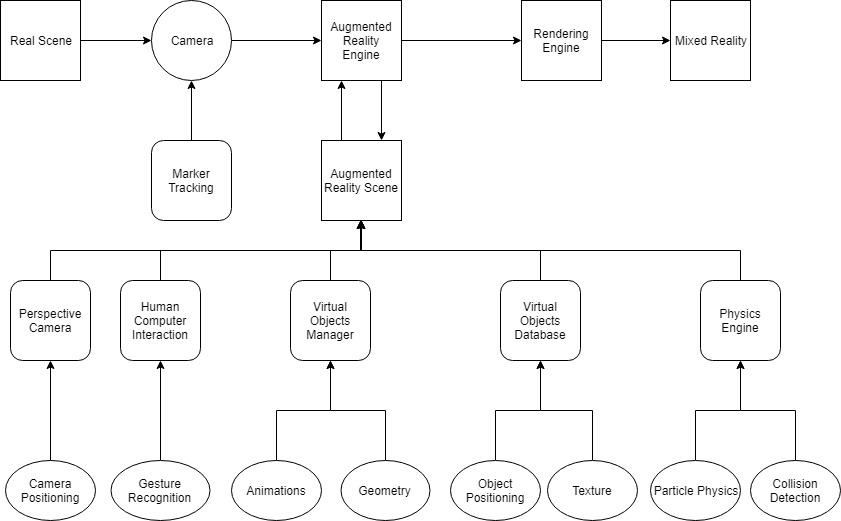
\includegraphics[width=\linewidth, height=10cm,keepaspectratio]{arch}
	\caption{System Architecture}
	\label{fig:arch}
\end{figure}

\section{Description}
The architecture diagram includes the main components of the AR application like Camera, AR Engine,Virtual Object Manager. The diagram shows that the camera captures the live feed and digital objects are super imposed on to the real scene using an augmented reality engine.

The AR engine is responsible for rendering and maintaining the virtual scene called AR scene. In an AR scene perspective camera, physics engine, virtual objects database play an important role in making the experience seem realistic and natural by providing animations, textures, lighting, shadows.

After the real scene is processed by the AR engine the Virtual scene is mapped on to the real world by using a marker there by rendering a mixed reality on the screen.
\begin{figure}
	\centering
	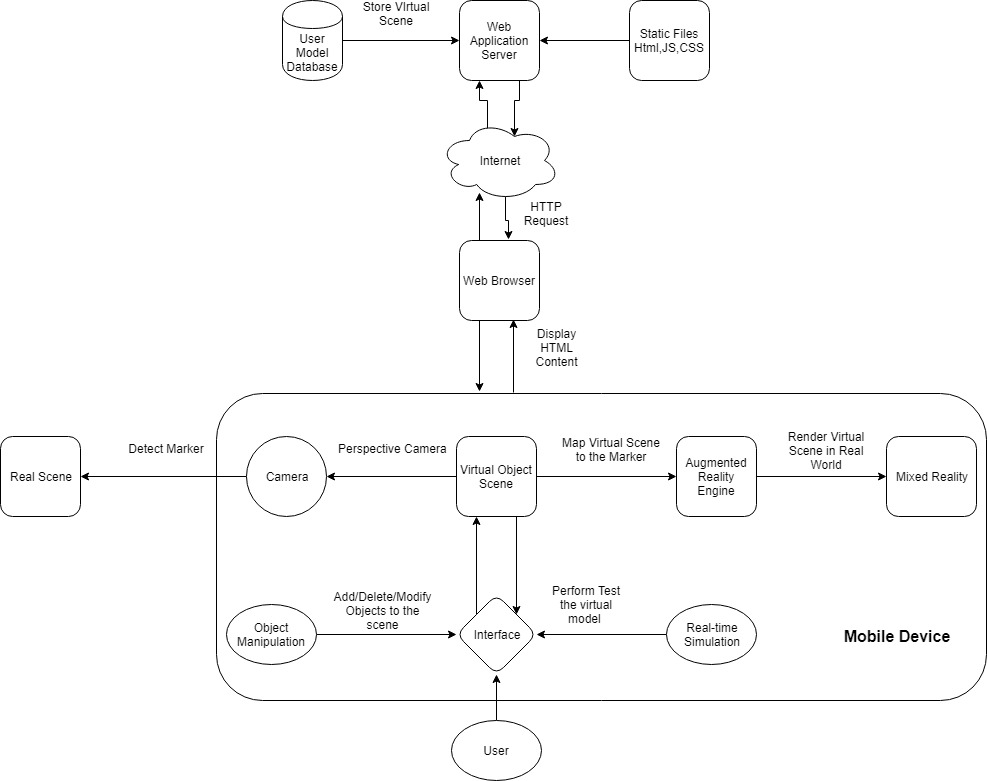
\includegraphics[width=\linewidth, height=10cm,keepaspectratio]{dataflow}
	\caption{DataFlow Diagram}
	\label{fig:data}
\end{figure}

In the data flow diagram the various modules and the process flow between these modules is comprehensibly described.
The data flow diagram shows the step by step process of the web application. First there will be a login page to validate user's credentials via a web browser, once the user enters the login information they will be taken to the restaurant's home page. The browser makes use of the device's camera to track the marker in the real world, Once marker position is established digital objects can be mapped into the real world.
The users can view their designs by visualizing the structure on their screen.

\section{System Requirements}
\subsection{Software specifications}
The software specifications required to build the software of the system are:
\begin{itemize}
	\item Web browser
	\item Node JS
	\item MongoDB
	\item HTML,CSS, JavaScript
	\item Blender
	\item GIT 
\end{itemize}
\subsubsection{JavaScript}
JavaScript often abbreviated as JS, is a high-level, interpreted programming language. It is a language which is also characterized as dynamic, weakly typed, prototype-based and multi-paradigm. Alongside HTML and CSS, JavaScript is one of the three core technologies of World Wide Web content engineering. It is used to make webpages interactive and provide online programs, including video games. The majority of websites employ it, and all modern web browsers support it without the need for plug-ins by means of a built-in JavaScript engine.
\subsubsection{WebGL}
WebGL is a cross-platform, royalty-free web standard for a low-level 3D graphics API based on OpenGL ES, exposed to ECMAScript via the HTML5 Canvas element. WebGL is integrated completely into all the web standards of the browser, allowing GPU-accelerated usage of physics and image processing and effects as part of the web page canvas. WebGL elements can be mixed with other HTML elements and composited with other parts of the page or page background. WebGL programs consist of control code written in JavaScript and shader code that is written in OpenGL Shading Language (GLSL), a language similar to C or C++, and is executed on a computer's graphics processing unit (GPU). 
\subsubsection{Node JS}
Node.js is an open-source, cross-platform JavaScript run-time environment that executes JavaScript code server-side. Historically, JavaScript was used primarily for client-side scripting, in which scripts written in JavaScript are embedded in a webpage's HTML and run client-side by a JavaScript engine in the user's web browser. Node.js lets developers use JavaScript for server-side scripting—running scripts server-side to produce dynamic web page content before the page is sent to the user's web browser. Consequently, Node.js represents a "JavaScript everywhere" paradigm unifying web application development around a single programming language, rather than different languages for server side and client side scripts.
\subsubsection{HTML}
Hypertext Markup Language (HTML) is the standard markup language for creating web pages and web applications. With Cascading Style Sheets (CSS) and JavaScript, it forms a triad of cornerstone technologies for the World Wide Web. Web browsers receive HTML documents from a web server or from local storage and render them into multimedia web pages. HTML describes the structure of a web page semantically and originally included cues for the appearance of the document.

HTML elements are the building blocks of HTML pages. With HTML constructs, images and other objects, such as interactive forms, may be embedded into the rendered page. It provides a means to create structured documents by denoting structural semantics for text such as headings, paragraphs, lists, links, quotes and other items. HTML elements are delineated by tags, written using angle brackets. Browsers do not display the HTML tags, but use them to interpret the content of the page.
\subsubsection{CSS}
Cascading Style Sheets (CSS) is a style sheet language used for describing the presentation of a document written in a markup language. Along with HTML and JavaScript, CSS is a cornerstone technology used by most websites to create visually engaging webpages, user interfaces for web applications, and user interfaces for many mobile applications.

CSS is designed primarily to enable the separation of presentation and content, including aspects such as the layout, colors, and fonts. This separation can improve content accessibility, provide more flexibility and control in the specification of presentation characteristics, enable multiple HTML pages to share formatting by specifying the relevant CSS in a separate .css file, and reduce complexity and repetition in the structural content.
\subsubsection{Git}
Git is a version control system for tracking changes in computer files and coordinating work on those files among multiple people. It is primarily used for source code management in software development, but it can be used to keep track of changes in any set of files. As a distributed revision control system it is aimed at speed, data integrity, and support for distributed, non-linear workflows.
\subsubsection{RESTful \ac{API}}
Representational state transfer (REST) or RESTful web services is a way of providing interoperability between computer systems on the Internet. REST-compliant Web services allow requesting systems to access and manipulate textual representations of Web resources using a uniform and predefined set of stateless operations.

An \ac{API} for a website is code that allows two software programs to communicate with each another.A RESTful \ac{API} explicitly takes advantage of HTTP methodologies. They use GET to retrieve a resource; PUT to change the state of or update a resource, which can be an object, file or block; POST to create that resource; and DELETE to remove it.
\subsubsection{\ac{JSON}}
JavaScript Object Notation or \ac{JSON} is an open-standard file format that uses human-readable text to transmit data objects consisting of attribute-value pairs and array data types (or any other serializable value). It is a very common data format used for asynchronous browser-server communication.

JSON is built on two structures:
A collection of name/value pairs. In various languages, this is realized as an object, record, struct, dictionary, hash table, keyed list, or associative array.
An ordered list of values. In most languages, this is realized as an array, vector, list, or sequence.
\subsubsection{AR.js}
Open Source,Efficient Augmented Reality for the Web. AR.js is a wrapper for three.js that performs well in mobile device.It is marker based. It supports a wide range of markers: multiple types of markers pattern/barcode multiple independent markers at the same 
\subsubsection{Three.js}
three.js is a cross-browser JavaScript library and Application Programming Interface (API) used to create and display animated 3D computer graphics in a web browser.
Three.js allows the creation of Graphical Processing Unit (GPU)-accelerated 3D animations using the JavaScript language as part of a website without relying on proprietary browser plugins. This is possible thanks to the advent of WebGL
\subsubsection{A-Frame.io}
A-Frame is an open-source web framework for building virtual reality (VR) experiences.It is primarily maintained by Mozilla and the WebVR community. It is an entity component system framework for Three.js where developers can create 3D and WebVR scenes using HTML. HTML provides a familiar authoring tool for web developers and designers while incorporating a popular game development pattern used by engines such as Unity.
\subsubsection{MongoDB}
MongoDB is a free and open-source cross-platform document-oriented database program. Classified as a NoSQL database program, MongoDB uses JSON-like documents with schemas. 

Using MongoDB removes the complex object-relational mapping (ORM) layer that translates objects in code to relational tables. MongoDB's flexible data model also means that your database schema can evolve with business requirements.
time, or multiple markers acting as a single marker up to you to choose.


\subsection{Hardware specifications}
The hardware specifications required by the system are:
\begin{itemize}
\item Dual-core or 64-bit processor
\item HQ Camera and input devices
\item Adreno 509 or higher GPU
\item Accelerometer, GPS, and solid state compass
\item Atleast 3 GB RAM
\end{itemize}
\section{Summary}
Thus the system design has been analyzed and a detailed description about the design of this system has been given in this chapter. The analysis of the design of the system gives the detailed overview about the project, in this chapter detailed description of each and every module is given which briefs the user about the various features and advantages of the project. This chapter has also given information about the available features and options in the project. The requirements of the system also have been given for the better understanding of the technology used in the project.

\chapter{Module Description}
\section{Introduction}
In this section, we're going to talk about the various modules in this project. We have divided the whole project into many sub sections and the three main modules of the project will be discussed below. Apart from discussing about it, the work flow diagram of each module is going to be provided to provide a clear idea of what the module is going to be and in-turn how the whole project is going to be.
\section{Login Module}
\begin{figure}[htbp]
	\centering
	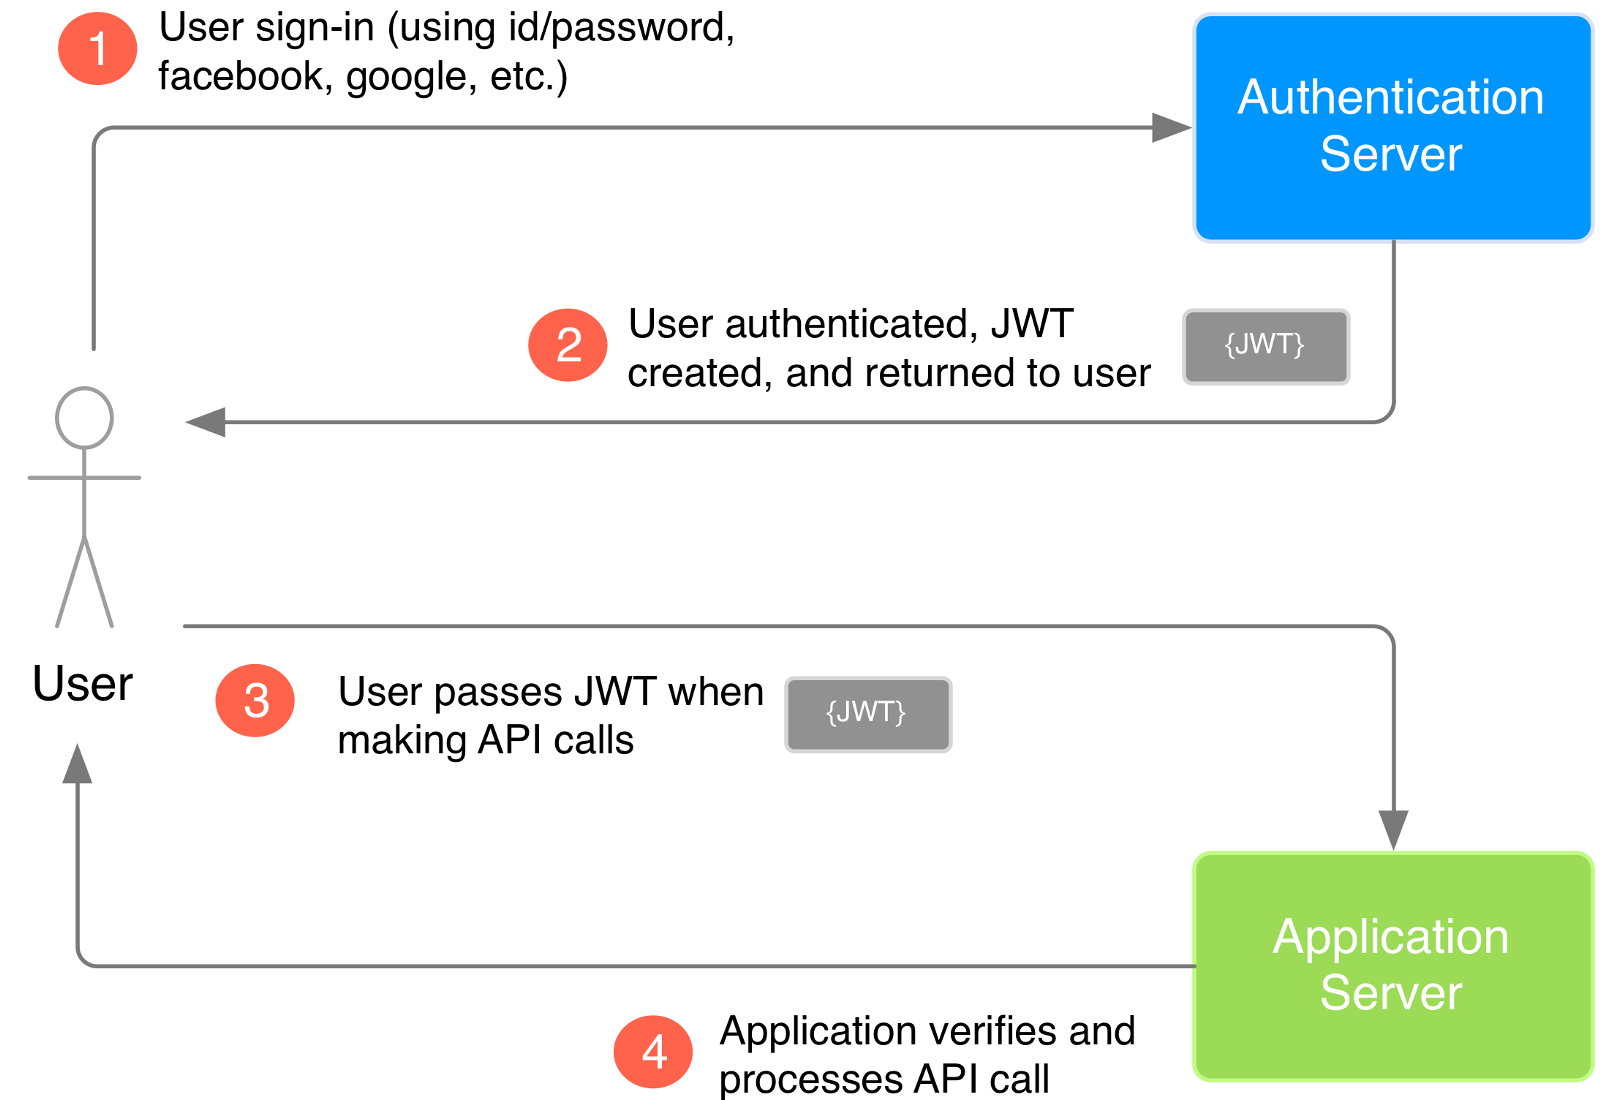
\includegraphics[width=\linewidth, height=7cm,keepaspectratio]{loginmodule}
	\caption{Work flow diagram for Login Module}
	\label{fig:loginmodule}
\end{figure} 
\paragraph{Description}
The log in is the most important part of the application as it  provides a layer of security to the app. The user will enter the email and password and based on the suffix of the email, the app will first authenticate the user and then redirect to the home page.JSON Web Tokens are used for representing claims securely between two parties.It is an open, industry standard for stateless authentication.
\section{Augmented Reality Scene}
\begin{figure}[htbp]
	\centering
	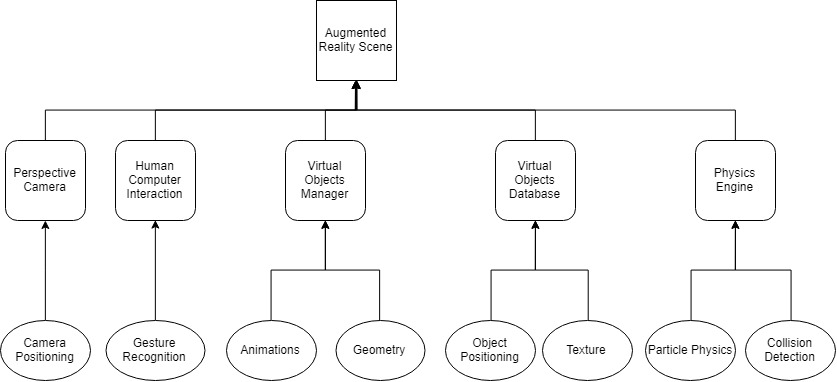
\includegraphics[width=\linewidth, height=7cm,keepaspectratio]{arscenemodule}
	\caption{Work flow diagram for AR Scene Module}
	\label{fig:hodmodule}
\end{figure} 
\paragraph{Description}
Scenes allow you to set up what and where is to be rendered by the rendering engine. This is where you place objects, lights and cameras.
\begin{itemize}
\item Perspective Camera
\item Human Computer Interaction
\item Virtual Object Manager
\item Virtual Object Database
\item Physics Engine
\end{itemize}
All this information is stored in the database and which is used to render the scene. 
\section{Marker Tracking}
Marker-based AR uses a Camera and a visual marker to determine the center, orientation and range of its spherical coordinate system. Using a marker makes the application run faster as the object to detect is known beforehand.
\section{Gesture Recognition}
Interaction with the digital environment via hand gestures makes the experience quick and natural. Gestures to scale, manipulate or rotate the 3D Scene gives the user a sense of freedom.
\section{3D Scene Rendering}
Rendering the virtual model using WebGL and mapping it on the marker. Visual artifacts like shadows, lighting, texture, and distance are added to the final render that is displayed on the screen.
\subsubsection{3D Object Interaction}
The real space is used for data input, users perform gestures that are detected by the camera in real-time and the 3D virtual scene is projected onto the real environment reflecting the changes made by the user.
\section{Summary}
As has been shown above, the project has been divided into 3 major modules and they have been explained in detail. The login module being the one that handles the security ,The AR scene module is responsible for rendering the virtual scene and the physics engine helps in simulation of objects in the scene.
\chapter{System Implementation}
\section{Introduction}
As the project should be easily accessible, We've developed it using Web Technologies so that it can run on any device that has a web browser and is not limited by OS or Hardware.
Since it is a web application no installation is required and can be accessed anywhere.
\section{Overview of the project environment}
\subsection{Collision detection}
Objects in games interact with the player, the environment, and each other. Typically, most 3D objects in games are represented by two separate meshes or shapes. One of these meshes is the highly complex and detailed shape visible to the player in the game, such as a vase with elegant curved and looping handles. For purpose of speed, a second, simplified invisible mesh is used to represent the object to the physics engine so that the physics engine treats the example vase as a simple cylinder. It would thus be impossible to insert a rod or fire a projectile through the handle holes on the vase, because the physics engine model is based on the cylinder and is unaware of the handles. The simplified mesh used for physics processing is often referred to as the collision geometry. This may be a bounding box, sphere, or convex hull. Engines that use bounding boxes or bounding spheres as the final shape for collision detection are considered extremely simple. Generally a bounding box is used for broad phase collision detection to narrow down the number of possible collisions before costly mesh on mesh collision detection is done in the narrow phase of collision detection.
\subsection{Soft-body dynamics}
An alternative to using bounding box-based rigid body physics systems is to use a finite element-based system. In such a system, a 3-dimensional, volumetric tessellation is created of the 3D object. The tessellation results in a number of finite elements which represent aspects of the object's physical properties such as toughness, plasticity, and volume preservation. Once constructed, the finite elements are used by a solver to model the stress within the 3D object. The stress can be used to drive fracture, deformation and other physical effects with a high degree of realism and uniqueness.


\subsection{Simulation Algorithm}
\makeatletter
\newcommand{\verbatimfont}[1]{\def\verbatim@font{#1}}%
\makeatother
\verbatimfont{\rmfamily}
\begin{verbatim}
<!DOCTYPE html>
<html lang="en">
<head>
<title>three.js webgl - shaders - ocean</title>
<meta charset="utf-8">
<meta name="viewport" content="width=device-width, user-scalable=no, minimum-scale=1.0, maximum-scale=1.0">
<style>

body {
	color: #000;
	font-family:Monospace;
	font-size:13px;
	margin: 0px;
	overflow: hidden;
}

#info {
	position: absolute;
	top: 0px; width: 100%;
	text-align:center;
	padding: 5px;
}

</style>
</head>
<body>

<div id="container"></div>
<div id="info">
<a href="http://threejs.org" target="_blank" rel="noopener">three.js</a> - webgl ocean
</div>

<script src="../build/three.js"></script>

<script src="js/controls/OrbitControls.js"></script>
<script src="js/objects/Water.js"></script>
<script src="js/objects/Sky.js"></script>

<script src="js/Detector.js"></script>
<script src="js/libs/stats.min.js"></script>
<script src="js/libs/dat.gui.min.js"></script>

<script>

if ( ! Detector.webgl ) Detector.addGetWebGLMessage();

var container, stats;
var camera, scene, renderer, light;
var controls, water, sphere;

init();
animate();

function init() {
	
	container = document.getElementById( 'container' );
	
	//
	
	renderer = new THREE.WebGLRenderer();
	renderer.setPixelRatio( window.devicePixelRatio );
	renderer.setSize( window.innerWidth, window.innerHeight );
	container.appendChild( renderer.domElement );
	
	//
	
	scene = new THREE.Scene();
	
	//
	
	camera = new THREE.PerspectiveCamera( 55, window.innerWidth / window.innerHeight, 1, 20000 );
	camera.position.set( 30, 30, 100 );
	
	//
	
	light = new THREE.DirectionalLight( 0xffffff, 0.8 );
	scene.add( light );
	
	// Water
	
	var waterGeometry = new THREE.PlaneBufferGeometry( 10000, 10000 );
	
	water = new THREE.Water(
	waterGeometry,
	{
		textureWidth: 512,
		textureHeight: 512,
		waterNormals: new THREE.TextureLoader().load( 'textures/waternormals.jpg', function ( texture ) {
			texture.wrapS = texture.wrapT = THREE.RepeatWrapping;
		}),
		alpha: 1.0,
		sunDirection: light.position.clone().normalize(),
		sunColor: 0xffffff,
		waterColor: 0x001e0f,
		distortionScale:  3.7,
		fog: scene.fog !== undefined
	}
	);
	
	water.rotation.x = - Math.PI / 2;
	
	scene.add( water );
	
	// Skybox
	
	var sky = new THREE.Sky();
	sky.scale.setScalar( 10000 );
	scene.add( sky );
	
	var uniforms = sky.material.uniforms;
	
	uniforms.turbidity.value = 10;
	uniforms.rayleigh.value = 2;
	uniforms.luminance.value = 1;
	uniforms.mieCoefficient.value = 0.005;
	uniforms.mieDirectionalG.value = 0.8;
	
	var parameters = {
		distance: 400,
		inclination: 0.49,
		azimuth: 0.205
	};
	
	var cubeCamera = new THREE.CubeCamera( 1, 20000, 256 );
	cubeCamera.renderTarget.texture.minFilter = THREE.LinearMipMapLinearFilter;
	
	function updateSun() {
		
		var theta = Math.PI * ( parameters.inclination - 0.5 );
		var phi = 2 * Math.PI * ( parameters.azimuth - 0.5 );
		
		light.position.x = parameters.distance * Math.cos( phi );
		light.position.y = parameters.distance * Math.sin( phi ) * Math.sin( theta );
		light.position.z = parameters.distance * Math.sin( phi ) * Math.cos( theta );
		
		sky.material.uniforms.sunPosition.value = light.position.copy( light.position );
		water.material.uniforms.sunDirection.value.copy( light.position ).normalize();
		
		cubeCamera.update( renderer, scene );
		
	}
	
	updateSun();
	
	//
	
	var geometry = new THREE.IcosahedronGeometry( 20, 1 );
	
	for ( var i = 0, j = geometry.faces.length; i < j; i ++ ) {
		
		geometry.faces[ i ].color.setHex( Math.random() * 0xffffff );
		
	}
	
	var material = new THREE.MeshStandardMaterial( {
		vertexColors: THREE.FaceColors,
		roughness: 0.0,
		flatShading: true,
		envMap: cubeCamera.renderTarget.texture,
		side: THREE.DoubleSide
	} );
	
	sphere = new THREE.Mesh( geometry, material );
	scene.add( sphere );
	
	//
	
	controls = new THREE.OrbitControls( camera, renderer.domElement );
	controls.maxPolarAngle = Math.PI * 0.495;
	controls.target.set( 0, 10, 0 );
	controls.panningMode = THREE.HorizontalPanning;
	controls.minDistance = 40.0;
	controls.maxDistance = 200.0;
	camera.lookAt( controls.target );
	
	//
	
	stats = new Stats();
	container.appendChild( stats.dom );
	
	// GUI
	
	var gui = new dat.GUI();
	
	var folder = gui.addFolder( 'Sky' );
	folder.add( parameters, 'inclination', 0, 0.5, 0.0001 ).onChange( updateSun );
	folder.add( parameters, 'azimuth', 0, 1, 0.0001 ).onChange( updateSun );
	folder.open();
	
	var uniforms = water.material.uniforms;
	
	var folder = gui.addFolder( 'Water' );
	folder.add( uniforms.distortionScale, 'value', 0, 8, 0.1 ).name( 'distortionScale' );
	folder.add( uniforms.size, 'value', 0.1, 10, 0.1 ).name( 'size' );
	folder.add( uniforms.alpha, 'value', 0.9, 1, .001 ).name( 'alpha' );
	folder.open();
	
	//
	
	window.addEventListener( 'resize', onWindowResize, false );
	
}

function onWindowResize() {
	
	camera.aspect = window.innerWidth / window.innerHeight;
	camera.updateProjectionMatrix();
	
	renderer.setSize( window.innerWidth, window.innerHeight );
	
}

function animate() {
	
	requestAnimationFrame( animate );
	render();
	stats.update();
	
}

function render() {
	
	var time = performance.now() * 0.001;
	
	sphere.position.y = Math.sin( time ) * 20 + 5;
	sphere.rotation.x = time * 0.5;
	sphere.rotation.z = time * 0.51;
	
	water.material.uniforms.time.value += 1.0 / 60.0;
	
	renderer.render( scene, camera );
	
}

</script>
</body>
</html>
\end{verbatim}
\begin{figure}[htbp]
	\centering
	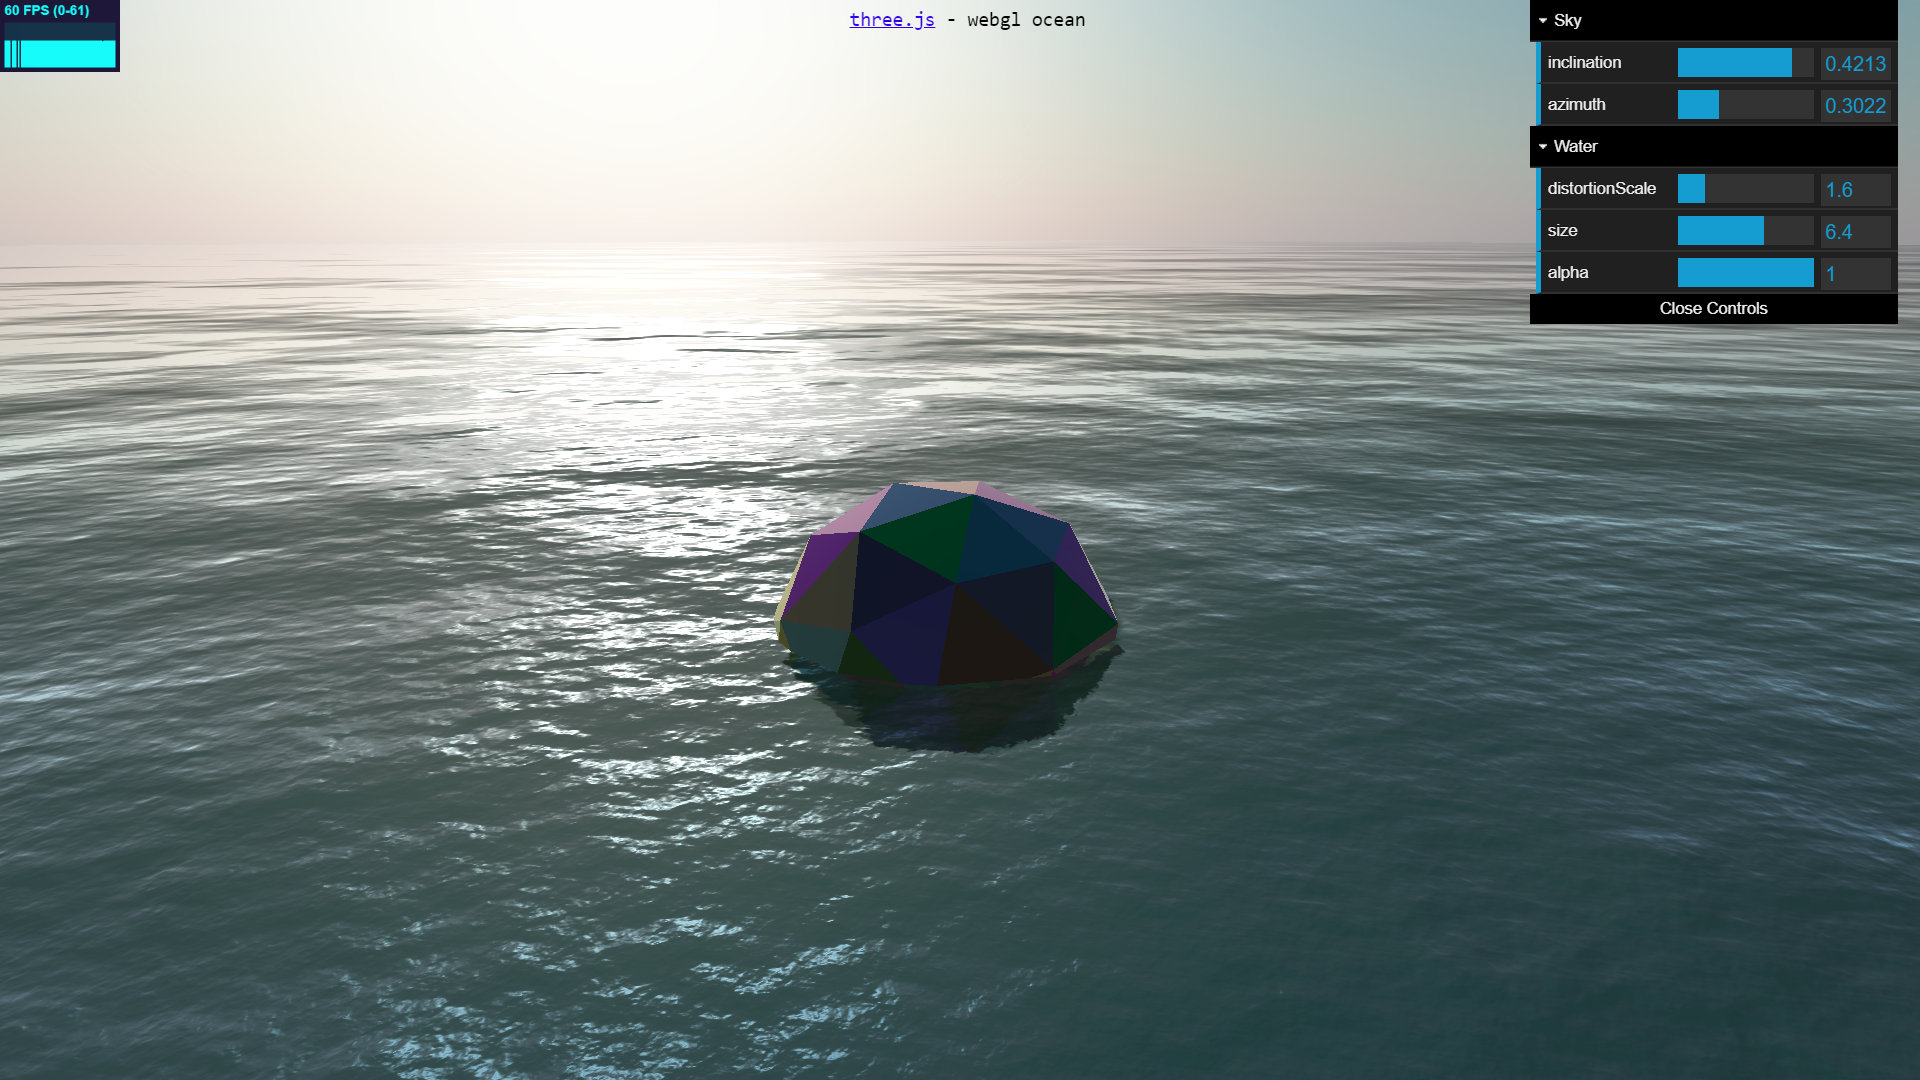
\includegraphics[width=\linewidth, height=10cm,keepaspectratio]{render}
	\caption{Object Interaction with water}
	\label{fig:arch}
\end{figure}
\begin{figure}[htbp]
	\centering
	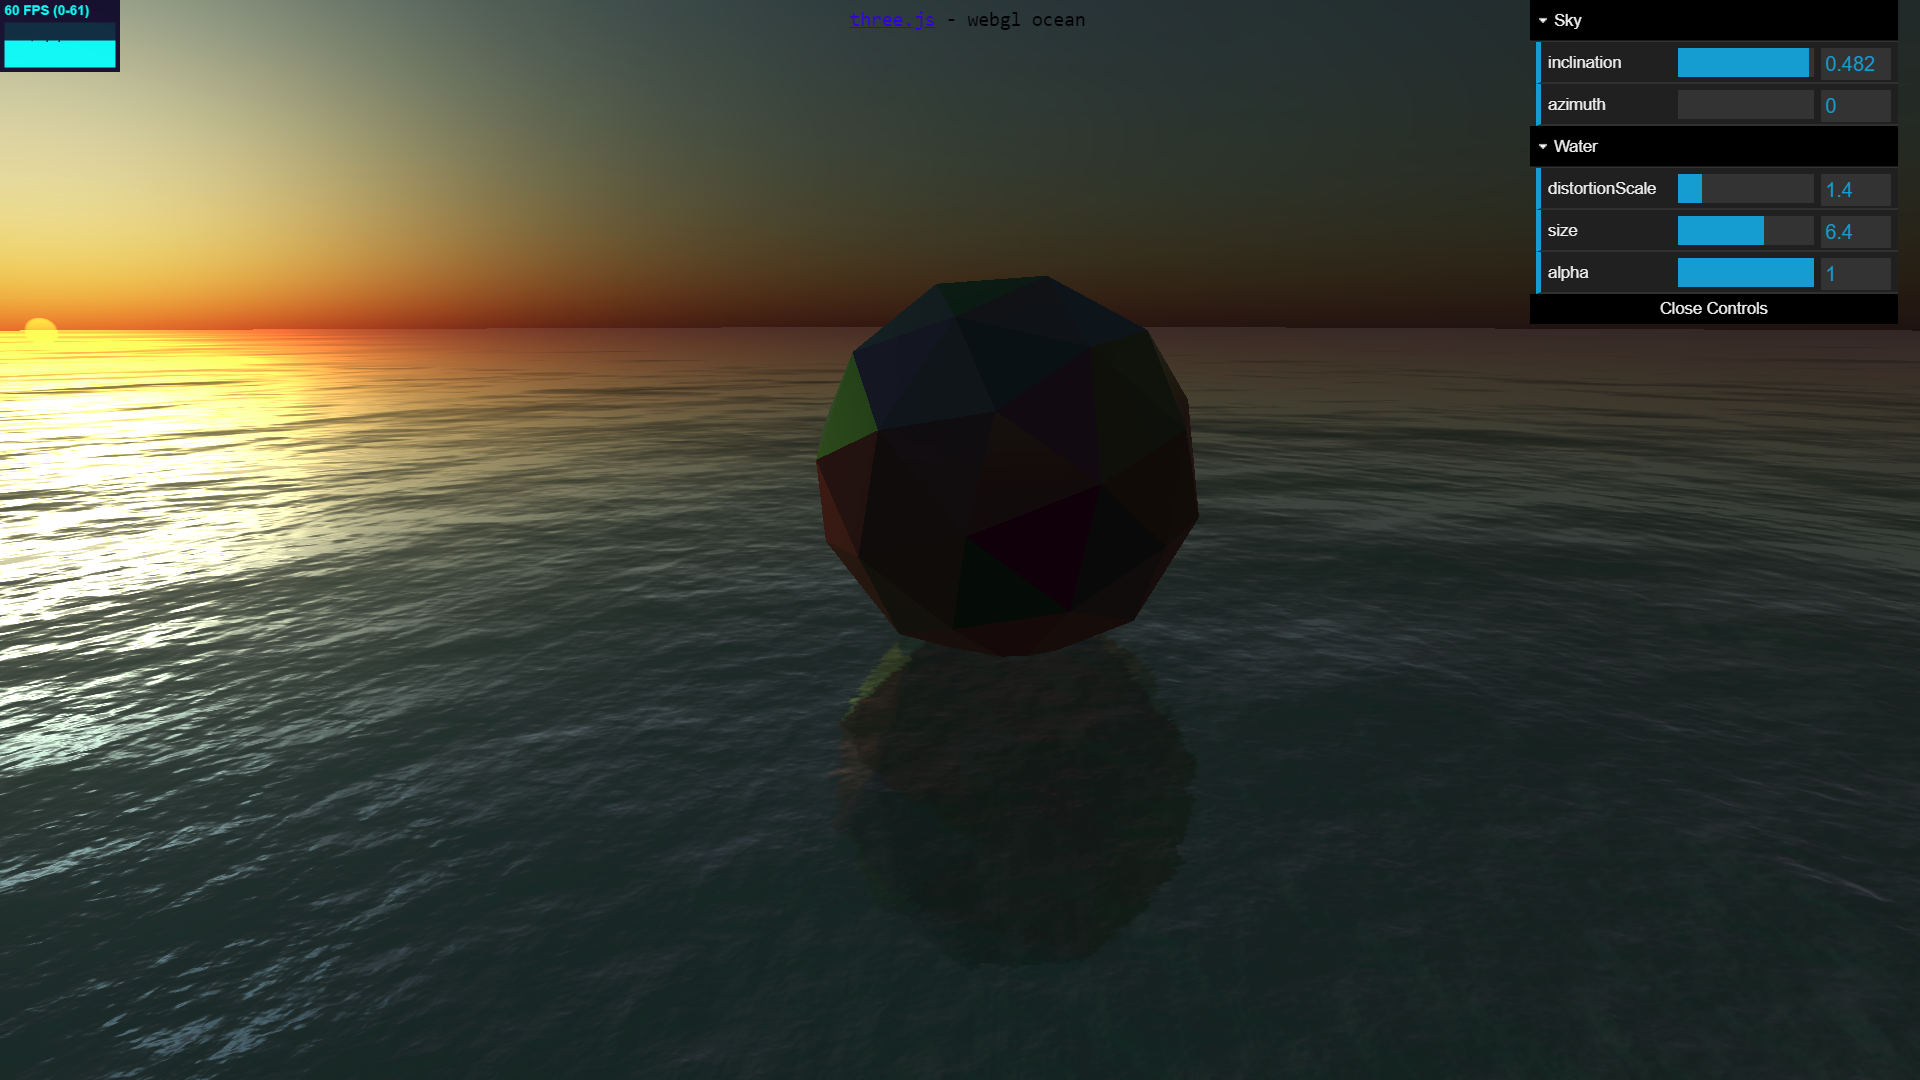
\includegraphics[width=\linewidth, height=10cm,keepaspectratio]{render2}
	\caption{Simulate Natural Light around the object}
	\label{fig:arch}
\end{figure}

\section{Performance Analysis}

\subsection{Simulation Parameters}
Web Testing in simple terms is checking your web application for potential bugs before its made live or before code is moved into the production environment.

During this stage issues such as that of web application security, the functioning of the site, its access to handicapped as well as regular users and its ability to handle traffic is checked.
\subsubsection{Unit Testing}
This is the first level of testing. In this different modules are tested against the specifications produced during the design of the module. During this testing the number of the arguments is compared to input parameters, matching of parameter and arguments etc. All five modules are checked separately, each test case is given to each unit and it is checked. The result is checked to see if the actual outcome is same as the expected outcome.A unit test is also called a module test because it tests the individual units of code that comprise the application. Each test validates a single module that was built to perform a certain task with the expectation that it will behave in a specific way. During this testing the number of the arguments is compared to input parameters, matching of parameter and arguments etc. All five modules are checked separately, each test case is given to each unit and it is checked. The result is checked to see if the actual outcome is same as the expected outcome.A unit test is also called a module test because it tests the individual units of code that comprise the application. Each test validates a single module that was built to perform a certain task with the expectation that it will behave in a specific way.
\subsubsection{Integration testing}
Integration testing is a process where all the separate modules are combined together
and its working is checked. There are two approaches to this : bottom-up and top-down
integration.At first the branch, semester and grade selection modules are integrated and checked.Top-down approach is being used in this software testing.
\subsubsection{User acceptance testing}
User acceptance of a system is the factor for the success of any system. The system
under consideration is tested for the user acceptance by constantly keeping in touch
with the prospective system user at the time of developing wherever required.
\begin{itemize}
\item Input screen design.
\item Output screen design.
\item Online message to guide the user.
\item Format of the reports and other outputs
\end{itemize}
\subsubsection{Functional Testing}
Functional testing ensures that the application is working as per the requirements. Most of the test conducted for this is driven by the user interface and call flow
\subsubsection{Performance Testing}
This testing process is undertaken to check the performance and behavior of the application under certain conditions such as low battery, bad network coverage, low available memory, simultaneous access to application's server by several users and other conditions. Performance of an application can be affected from two sides:application's server side and client's side. Performance testing is carried out to check both.
\subsubsection{Memory Leakage Testing}
Memory leakage happens when a computer program or application is unable to manage the memory it is allocated resulting in poor performance of the application and the overall slowdown of the system. As mobile devices have significant constraints of available memory, memory leakage testing is crucial for the proper functioning of an application
\subsubsection{Interrupt Testing}
 An application while functioning may face several interruptions like incoming calls or network coverage outage and recovery. The different types of interruptions are:
\begin{itemize}
\item Incoming and Outgoing SMS and MMS
\item Incoming and Outgoing calls
\item Incoming Notifications
\item Battery Removal
\item Cable Insertion and Removal for data transfer
\item Network outage and recovery
\item Media Player on/off
\end{itemize}
An application should be able to handle these interruptions by going into a suspended state and resuming afterwards.
\subsubsection{Usability testing}
Usability testing is carried out to verify if the application is achieving its goals and getting a favorable response from users. This is important as the usability of an application is its key to commercial success (it is nothing but user friendliness).Another important part of usability testing is to make sure that the user experience is uniform across all devices.This section of testing hopes to address the key challenges of the variety of mobile devices and the diversity in mobile platforms/OS, which is also called device fragmentation. One key portion of this type of usability testing is to be sure that there are no major errors in the functionality, placement, or sizing of the user interface on different devices.
\subsubsection{Installation testing}
Certain mobile applications come pre-installed on the device whereas others have to be installed from the store. Installation testing verifies that the installation process goes smoothly without the user having to face any difficulty. This testing process covers installation, updating and uninstalling of an application
\subsubsection{Security Testing}
Security Testing: To check for vulnerabilities to hacking, authentication and authorization policies, data security, session management and other security standards.
\subsubsection{Results}
\begin{table}[htbp]
	\centering
\begin{tabular}{|L|L|L|c|}

	\hline
	Testing Parameters & Expected Output  & Actual Output &Result\\
	\hline
		\hline
	Authentication & Authenticate user by validating credentials from \ac{API} & User is Authenticated &Pass\\
		\hline
	Initialize Scene & Initialize the AR environment\ac{API} & AR scene initialized &Pass\\
		\hline
	Marker Tracking & Track marker position in the camera feed & Marker detected &Pass\\
		\hline
	AR Scene &  Fetch 3D model and render & Model rendered on the marker & Pass\\
		\hline
	Simulate Natural Calamities & Perform realistic simulations of natural calamities & Tests performed on the model &Pass\\
		\hline
	Analysis Report & Provide insights on the structure& Report of structural weak points provided &Pass\\
		\hline

\end{tabular}
\caption{Test-Cases}
\label{tab:test-cases}
  \end{table}
\begin{table}[htbp]
	\centering
\begin{tabular}{|c|L|c|}
	\hline
	Name of Test & Web Browsers & Test Result\\
	\hline
		\hline
	Unit testing & Chrome, Firefox, Safari & Pass\\
		\hline
	Integration testing & Chrome, Firefox & Pass\\
		\hline
	User Acceptance testing & Chrome, Firefox & Pass\\
		\hline
	Functional testing & Chrome, Firefox & Pass\\
		\hline
	Usability testing & Chrome, Firefox & Pass \\
		\hline
	Memory Leakage testing & Chrome, Firefox & Pass\\
		\hline
	Performance testing   & Chrome, Firefox & Pass\\
		\hline
	Interrupt testing & Chrome, Firefox & Pass\\
		\hline
	Installation tests & Chrome, Firefox & Pass\\
		\hline
	Security Testing & Chrome, Firefox& Pass\\
	
	\hline
\end{tabular}
\caption{Test-Results}
\label{tab:test-results}
\end{table}

\section{Summary}
The web application, incorporating the Restaurant Menu using Augmented Reality, is a very effective tool
which can be used for improving the overall efficiency in a Restaurant.During these tests, the number of arguments are compared to input parameters, matching of parameters and arguments etc.

The Application was tested on a web browser which lets you prototype, develop and test web applications without using a physical device. The application performed extremely well in low resource environments where the storage space and network connection is slow. Memory leaks were detected and resolved during development using performance profiling and code obfuscation ,optimization has been done.


\chapter{Conclusion and future enhancement}
\section{Conclusion}
Humans are visual creatures, therefore
a web application, incorporating augmented reality in construction, is a very effective tool which can be used for improving the overall efficiency in the design process.
This project proposes a method of application of physics engine to perform realistic simulations to the architectural design in AR environment that allows the user to interact with ease.

In this paper, we have included several test cases for simulating the natural calamities on the design that helps in providing an in-depth analysis of the structural weak points. Based on this report we can then improve our design by altering the materials or layout of the structure.To realize physical interactions different physical attributes like structural integrity, gravity and dynamics are taken into consideration. 
The proposed web application portability and ease in use
increases its credibility compared to the traditional system.
\section{Future Enhancement}
In the future gesture recognition techniques for placing 3D objects in AR environment can make the experience more interactive and realistic.
Since simulations are very resource intensive tasks the performance can be improved in future by rendering the simulation using server-side GPU computing.

Thus the application of AR in the field of architecture, structural design will eventually be useful to the Architects, Students as the design process is more interactive and helps in creating high-quality designs that can be visualized as if it was present in the real world.

% Bibliography.
\bibliographystyle{unsrt}
\bibliography{references}
%%%%%%%%%%%%%%%%%%%%%%%%%%%%%%%%%%%%%%%%%%%%%%%%%%%%%%%%%%%%
\end{document}
